%% ----------------------------------------------------------------
%% Requirements.tex
%% ---------------------------------------------------------------- 
\chapter{Requirements for the Forum Visualisation Tool} \label{Chapter:Requirements}

This chapter first gives a brief introduction of the SCN forum, and discusses the data model defined in the database. Secondly, the scope of the forum visualisation tool is limited with a tailored data model. Thirdly, a scenario consists of four interconnected use cases will be depicted based on the risk management. Lastly, a set of requirements derived from the scenario are listed.

\section{Data Model} \label{sec:data_model}
The SAP Community Network (SCN) is a professional social network hosted by SAP, which connects its customers, developers, employees, experts, and partners together.  It provides intimate knowledge of SAP products, solutions, and services. It also encourages the community users to generate and share rich content such as forum posts, weblogs, wikis, and articles in a collaborative environment. This thesis will focus on analysing and visualising data in the SCN forum.

\begin{figure}[!htb]
  \centering
  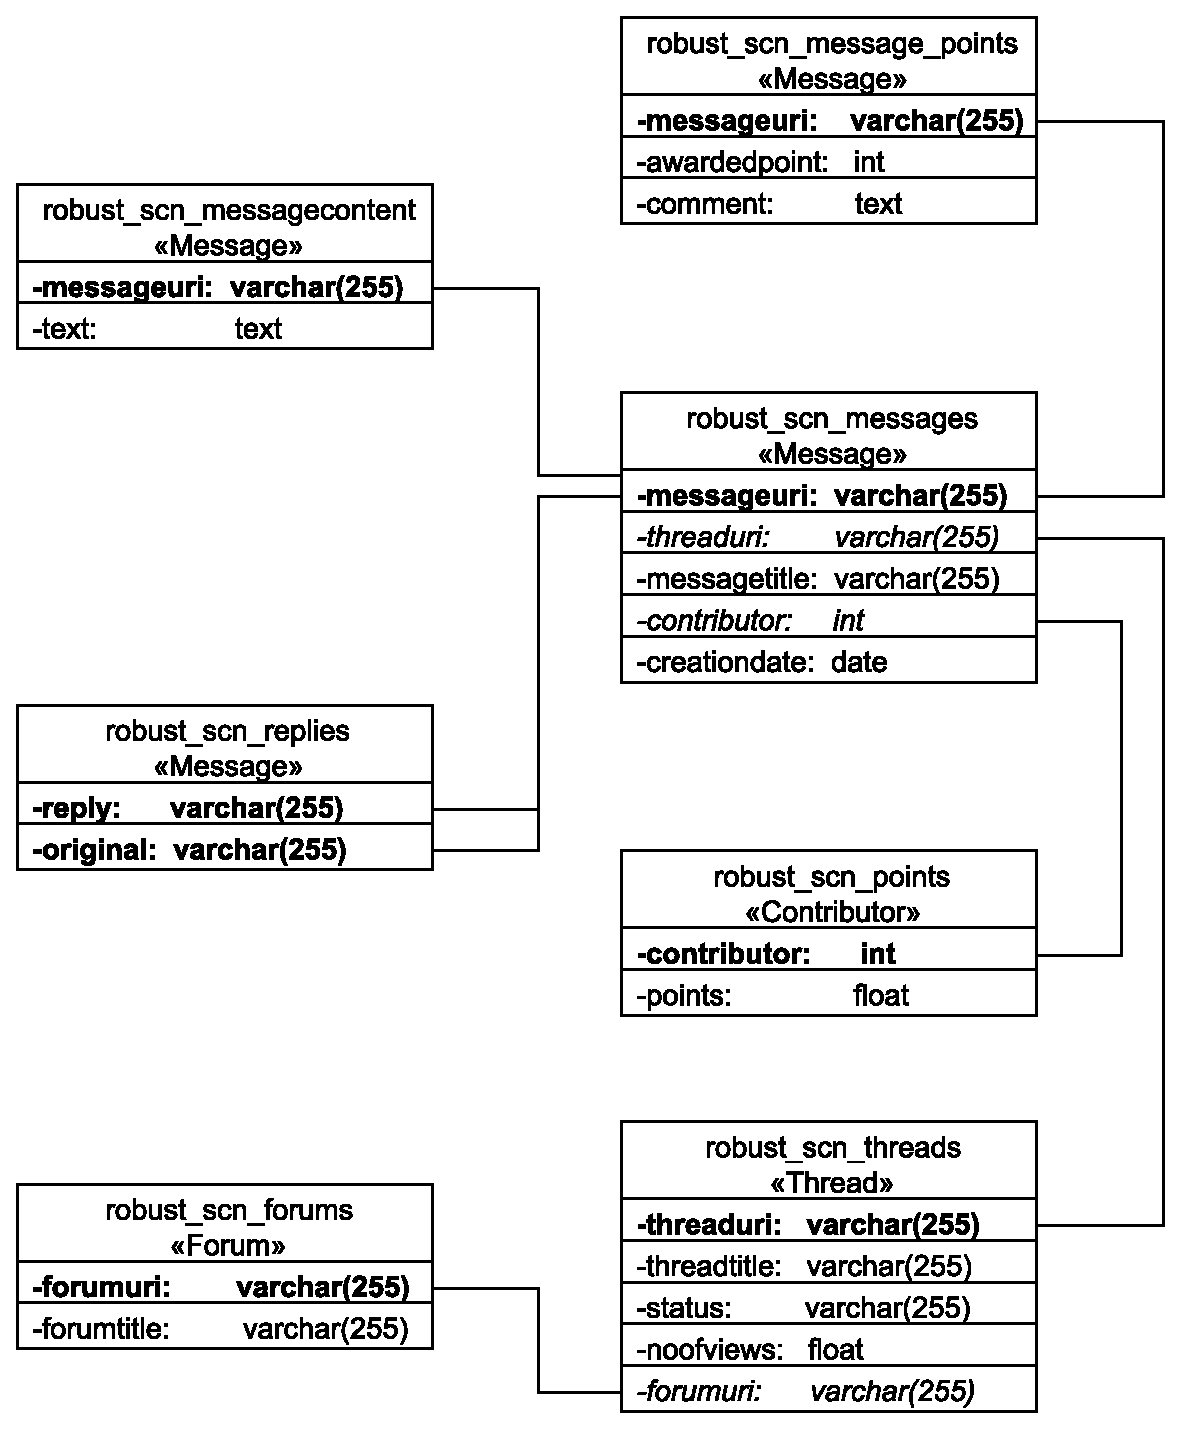
\includegraphics[scale=0.6]{05_01_relational_data_model.eps}
  \caption{The relational data model for the SAP Community Network forum.}
  \label{Figure:05_01}
\end{figure}
\fref{Figure:05_01} presents the relational data model of the SCN forum provided by SAP as a business partner use case of the ROBUST project \citep{Adrian2011}. The data model consists of four entities: the forum, contributor, thread, and message. The following is a full explanation of all fields in these entities. In addition, several important concepts based on the data model will be also defined for later used.

\textbf{Contributor.}~Defined in the \emph{robust\_scn\_points} data table, the \emph{contributor} refers to a contributor. The contributor field uniquely identifies a particular contributor. SAP does not provide the nicknames because of data privacy restraints, so each contributor will be labelled with the contributor field in the user interface. The \emph{points} field refers to the accumulated points this contributor has ever been awarded in the last twelve months and will be changed over time.

\textbf{Forum.}~Defined in the \emph{robust\_scn\_forums} data table, the forums refers to a collection of groups hierarchically organised to help contributors find their interesting discussions to participate in. For example, the SAP Business One SDK forum mainly includes something relevant to this specific discussion. The \emph{forumuri} field uniquely identifies a tuple in the table, while the \emph{forumtitle} field indicates the name of this forum. It should be noticed that forums are persistent although their content may change over time.

\textbf{Thread.}~Defined in the \emph{robust\_scn\_threads} data table, the thread refers to a series of messages concerning the same topic. The \emph{threaduri} field uniquely identifies a tuple in the table, while the \emph{threadtitle} field indicates the name of this thread. The \emph{forumuri} field defines the forum this thread belongs to. The status field indicate the current status of this thread and possible values includes `answered' and `unanswered'. The \emph{noofviews} field refers to the number of views of this thread.

\textbf{Message.}~The message refers to a written piece of information posted by a contributor, which is the building block of the SCN forum. Generally speaking, messages describes the post relationship between contributors and threads, which forms the basic activity in the SCN forum.

The main fields of messages are defined in the \emph{robust\_scn\_messages} data table. The \emph{messageuri} field uniquely identifies a tuple in the table, while the \emph{messagetitle} field indicates the name of this message. The \emph{threaduri} field defines the thread this message belongs to. The \emph{contributor} field shows the contributor of this message, which corresponds to the field with the same name in the \emph{robust\_scn\_points} data table. The \emph{creationdate} field refers to the time point when this message has been created.

The original message and reply message are defined as the \emph{original} and \emph{reply} field in the \emph{robust\_scn\_replies} data table, respectively. The latter is any message within a thread which replies to the former. Both correspond to the \emph{messageuri} field in the \emph{robust\_scn\_messages} data table. In addition, the SCN forum supports further nesting where an original message may be the reply message of another. From this point of view, each thread consists of a top-level message which is the first original message in chronological order, as well as a number of messages which directly or indirectly reply to the top-level message. The contributor who posts the top-level message is termed the \emph{original poster} of the thread and usually addresses an issue or asks a question.

Points can be awarded to contributors for each message. The \emph{robust\_scn\_message\_points} data table defines the amount of message points and the description in the \emph{awardedpoints} and \emph{comment} fields, respectively. And the \emph{messageuri} field is used to connect the field with the same name in the \emph{robust\_scn\_messages} data table. Specifically, the original poster of a thread has the right to give points to reply messages: two points for a helpful answer which can be awarded unlimited times within this thread, six points for a very helpful answer which can be awarded twice, and ten points for a solved problem which can be awarded only once. The message which has been awarded some message points is termed \emph{awarded message}. One contributor may be awarded multiple times by posting multiple useful reply messages within a thread.

The \emph{text} field in the \emph{robust\_scn\_messagecontent} data table defines the actual textual content of the message, whilst the \emph{messageuri} field is used to link to the field with the same name in the \emph{robust\_scn\_messages} data table.

\textbf{Snapshot.}~The term snapshot, which is not included in the relational data model, refers to a snapshot of a forum state during a given period of time. The \emph{start} and \emph{end} attributes will be added as the start and end timestamps, respectively. As a consequence, each forum can be divided into a set of fractions.

\subsection{The Scope of the Work} \label{sec:scope}
The scope of the forum visualisation tool is strictly limited to the visual representation of contributors, messages, and threads in the snapshot and will not take into account the following issues:
\begin{itemize}
  \item The reply network in the snapshot;
  \item The semantic of the message textual content;
  \item The network among different forums;
  \item The evolution of the forum by contrasting a series of continuous snapshots;
  \item The simulation that attempts to predict the future state of the forum.
\end{itemize}

\subsection{Tailored Data Model}
Having defined the scope of the work, it is important to note that the relational data model shown in \fref{Figure:05_01} should be tailored by removing several unused data tables as well as adding the snapshot entity. In addition, there is another reason to do so: the tailored data model should not be coupled with a particular Internet forum. Instead, a more generic data structure is needed to guarantee it still works well when the concrete data has changed.

\fref{Figure:05_02} illustrates the tailored data model in the form of the class diagram. The \emph{Snapshot} class is designed as a subclass of the \emph{Forum} class by adding the \emph{start} and \emph{end} attributes to specify a given period of time. The data collection in the snapshot is organised in a hierarchical structure. All attributes in the \emph{Contributor}, \emph{Message} and \emph{Thread} class are mapped to the fields with the same name in the \emph{robust\_scn\_points}, \emph{robust\_scn\_messages}, and \emph{robust\_scn\_threads} data tables, respectively. However, it should be noticed that two changes have been made. Firstly, the \emph{messagepoints} field in the \emph{robust\_scn\_message\_points} data table is merged into the Message class while the \emph{comment} field has been removed. Secondly, the \emph{points} attribute in the \emph{Contributor} class refers to the accumulated points this contributor has ever been awarded in the snapshot.

From a high-level view, each snapshot which inherits from a particular forum has zero or multiple threads. Each thread must belong to an instance of the \emph{Forum} class but may not be a part of any snapshot. Each message which belongs to an object of the \emph{Thread} class has only one contributor. Additionally, the \emph{AwardedMessage} class is a subclass of the \emph{Message} class in which the \emph{awardedpoints} attribute of any instance in this class must be greater than zero.

\begin{figure}[!htb]
  \centering
  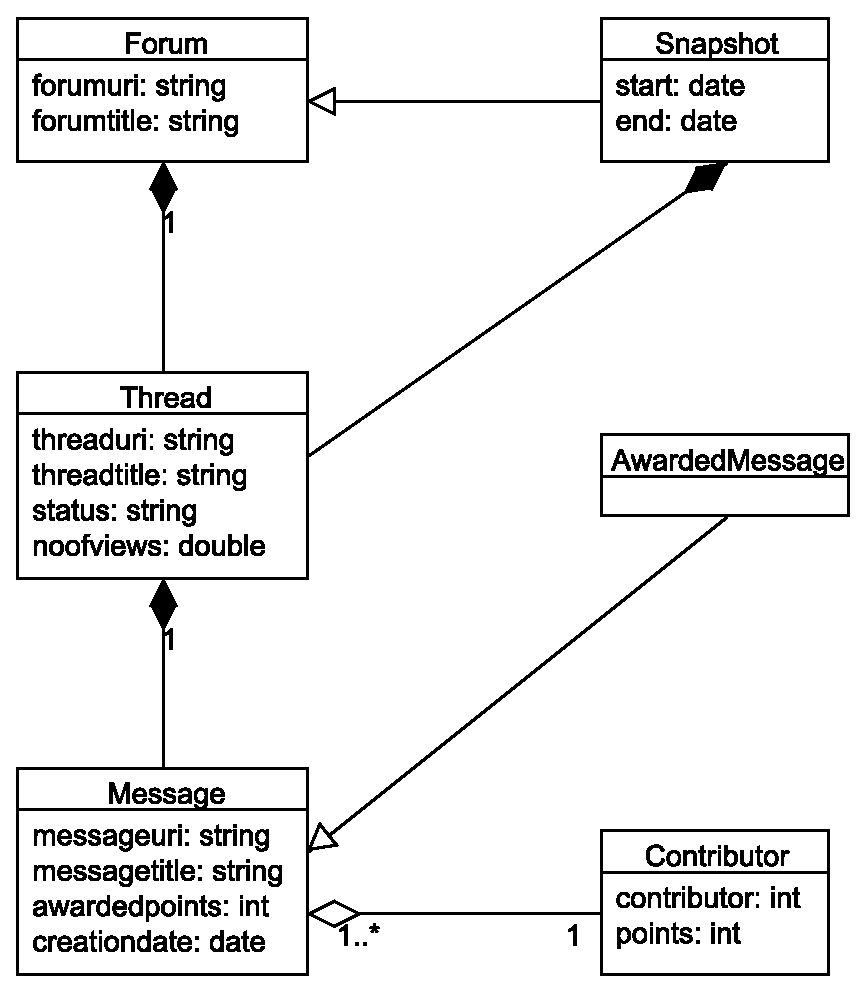
\includegraphics{05_02_class_diagram.eps}
  \caption{The class diagram for the forum visualisation tool.}
  \label{Figure:05_02}
\end{figure}

\section{Scenario} \label{sec:scenario}
This section depicts domain-specific user requirements of the forum visualisation tool in the form of the scenario  in \fref{Figure:05_03}. First of all, actors who make use of the forum visualisation tool should be identified among possible end users. Then the key scenario which details the steps of the interaction between actors and the forum visualisation tool will be clearly defined based on the risk management.

\begin{figure}[!htb]
  \centering
  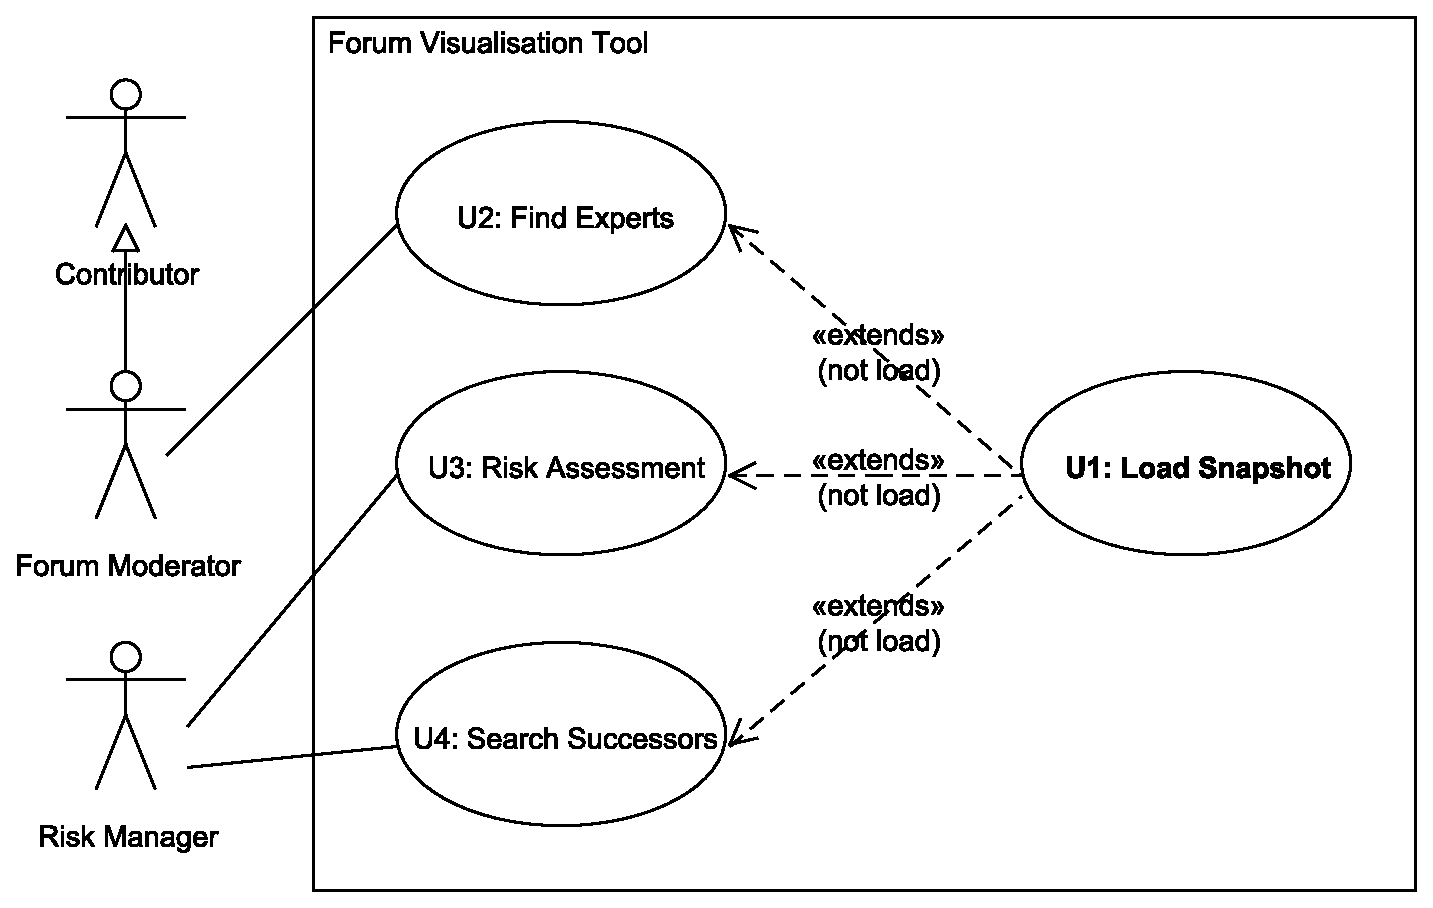
\includegraphics[scale=0.6]{05_03_use_case_diagram.eps}
  \caption{The use case diagram which includes four use cases.}
  \label{Figure:05_03}
\end{figure}

\subsection{Actors}
There are three different actors involved in the diagram: contributors, forum moderators, and risk managers. Contributors are not expected to use the forum visualisation tool directly because it is too professional for them. As a result, there is no link between contributors and any use case in the diagram. However, there is also a chance for them to make use of it in another way. The forum may share the visualisation generated by the forum visualisation tool with contributors to let them know their positions in order to encourage self-reflection.

The forum moderators are particular contributors whose primary responsibility is to promote interaction between contributors and make the forum more active. For instance, they regularly post top-level messages to add new content to the forum. The forum moderator is expected to be involved in the \emph{Find Experts} use case.

The risk managers identify any potential risk which may do harm to the forum. They are also responsible for deciding how to reduce risks if they really occurred. The risk manager is expected to be involved in the \emph{Risk Assessment} and \emph{Search Successors} use cases.

\subsection{Scenario Description}
The forum moderator intends to find out the top three experts in a given snapshot and then assign the risk manager to a task of risk assessment. Then, the risk manager receives the task and evaluates the risk by prioritise them in a reasonable order. Lastly, the risk manager completes the task by searching three potential successors who have the most similar expertise to each leaving expert, for the purpose of reducing the risk.

\subsection{Technical Description} \label{sec:tech_desc}
First of all, it is important to note that there is an implicit use case in the scenario. The \emph{Load Snapshot} use case will be only included in the \emph{Find Experts}, \emph{Risk Assessment}, and \emph{Search Successors} use cases under the condition when the snapshot data has not been loaded. Thus the snapshot data is cached in the memory once loaded from the data source.

As defined in \citep{Mcdonald2000}, an expert is a contributor who has much knowledge to answer a particular problem or moves the question toward the final resolution somehow. Apparently, this definition is twofold. In the case of the SCN forum, any contributor who has completely solved the question would be awarded ten points, while the one who has posted a helpful or very helpful answer would gain two or six points as a reward for providing useful information. Because the semantic of message content is beyond the scope of the work (see Section~\ref{sec:scope}), the awarded points of each message can be considered as the only metric to measure the quality of this message based on the assumption that the points are awarded fairly and consistently by the original poster. The more points awarded to a message, the more expertise provided from this message.

Building on the awarded points of each message, the Contributor Recognition Program (CRP)\footnote{http://www.sdn.sap.com/irj/scn/crphelp} has been developed by SCN as a level-based point system to measure the expertise of contributors. There are two distinct accumulated points for each contributor: lifetime points and annual points. The former refers to the number of points a contributor has ever been awarded since the registration date, while the latter refers to the points that a contributor has accumulated in the last twelve months on a rolling period. CRP is based on the annual points, since the SCN forum encourages contributors to contribute regularly to maintain their annual points over the rolling twelve months. Lastly, the five leading contributors in each specific forum on SCN will be displayed on the Find the Expert\footnote{http://www.sdn.sap.com/irj/scn/leadingcontributors} page.

Having discussed the strategy used in CRP, a conclusion can be drawn that the expertise of a specific contributor is proportional to the accumulated points she has ever been awarded in the snapshot for the duration of twelve months. With respect to the forum visualisation tool, an algorithm for calculating the expertise for each contributor is employed, which represents two minor differences compared with CRP. Firstly, it is possible to find experts over a flexible period of time. Secondly, the number of top experts decreases from five to three.

In this scenario, the process of the risk management has been simplified into three steps. Firstly, once the top three experts in a given snapshot have been identified by a forum moderator, a risk manager is assigned the task of the risk assessment. Secondly, this risk manager prioritises these risks in terms of the risk impact and likelihood attributes. The former refers to a possibility that the risk of experts leaving is reasonably expected to happen, while the latter represents the influence over the forum if this risk occurs. It is possible for an influential expert to walk out of the forum without any indication, which results in a big loss to the forum. Hence the priority of each risk can be defined by the combination of the likelihood and the impact. For example, an expert who has not only a strong possibility of leaving the forum but also a major impact upon her leaving should be put first. Finally, this risk manager is also in charge of seeking the treatment to reduce this risk by searching three potential successors to each expert.

\section{Use Cases} \label{sec:use_cases}
\fref{Figure:05_04} depicts the scenario in a time sequence of use cases. The key use cases are shown using red arrows, while the return values are optionally indicated using a dashed arrow. Especially, the \emph{Assign Task} use case is excluded in \fref{Figure:05_03}, because it is beyond the boundaries of the forum visualisation tool.

\begin{figure}[!htb]
  \centering
  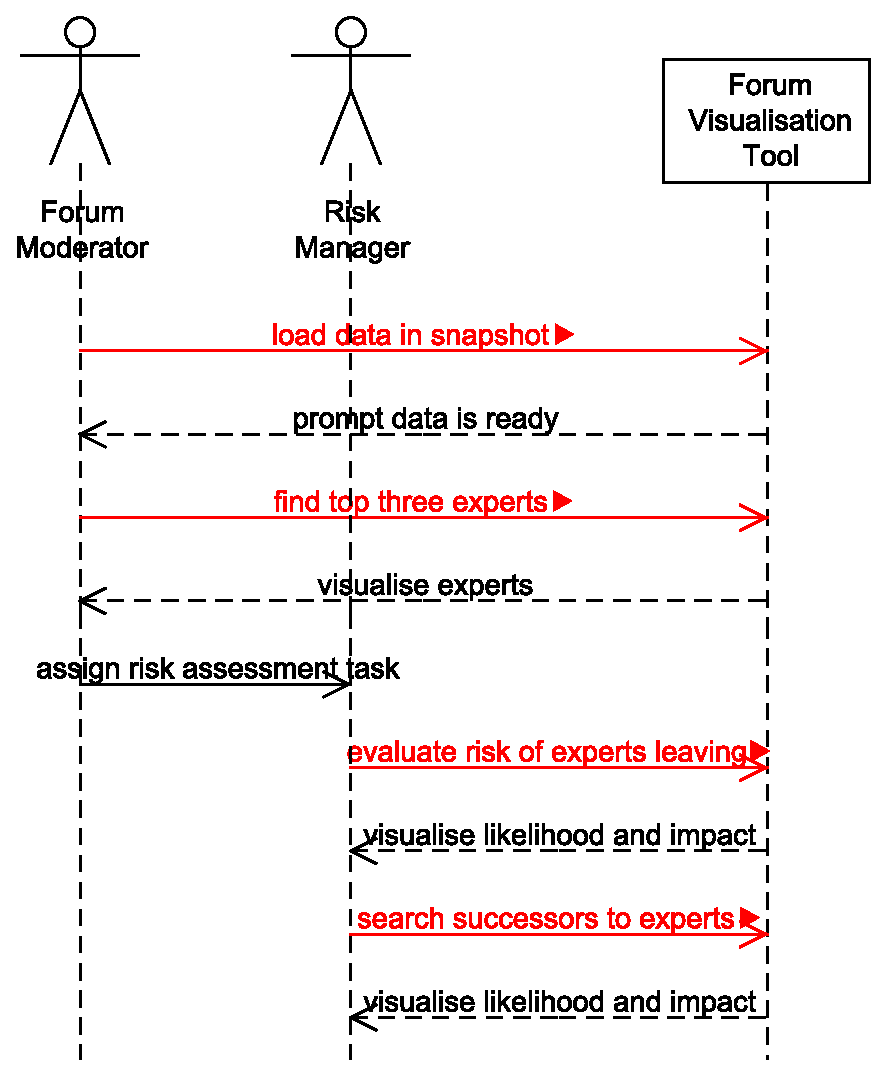
\includegraphics{05_04_sequence_diagram.eps}
  \caption{The sequence diagram depicts the scenario in a time sequence of use cases.}
  \label{Figure:05_04}
\end{figure}

\textbf{U1: Load Snapshot.}
The \emph{Load Snapshot} use case receives a period of time and a forum as input, and then returns a collection of data associated with the given snapshot.

\textbf{U2: Find Experts.}
The \emph{Find Experts} use case receives a specific snapshot as input, and then returns a graph visualisation showing the top three experts in the given snapshot under the condition that the data in the snapshot has been loaded and cached in the memory.

\textbf{U3: Risk Assessment}
The \emph{Risk Assessment} use case receives an expert and a snapshot as input, and then returns a graph visualisation showing the risk impact and likelihood under the condition that the data in the snapshot has been loaded and cached in the memory.

\textbf{U4: Search Successors}
The \emph{Search Successors} use case receives an expert and a snapshot as input, and then returns a graph visualisation showing the three potential successors to this expert under the condition that the data in the snapshot has been loaded and cached in the memory.

\section{Requirements} \label{sec:requirements}
This section summarises requirements derived from the scenario as discussed in Section~\ref{sec:scenario}. The scenario is intended to be described in an ambiguous way in order to separated it from the design and implementation of the forum visualisation tool. This section emphasises concrete requirements captured in the use cases.

\textbf{R1: General Requirements for Graph Visualisation.}
The forum visualisation tool must provide the following general requirements as infrastructure facilities for graph visualisation: navigation, interaction, built-in layout, visual properties, filtering, highlighting, clustering, satellite view, and dynamic graph. Several relevant studies have been reported in the literature. \citep{Noik1992} outlines a set of requirements which are common for graph visualisation software. Recently, a thorough list of general requirements for modern graph visualisation software has been defined in \citep{Zabiniako2009}, where the author lists more than forty concrete requirement derived from fifteen high-level requirements.

\textbf{R2: Contributor-to-Contributor Graph Visualisation.}
A contributor-to-contributor graph visualisation must be offered to present the expertise of contributors as well as the common expertise among them. This graph visualisation is the building block of the forum visualisation tool, and plays a pivot role in the \emph{Find Experts}, \emph{Risk Assessment}, and \emph{Search Successors} use cases.

First of all, this graph visualisation must provide a way for forum moderators to find the top three experts in a global perspective. Technically, contributors are expected to be rendered as nodes to represent an entity, whilst the common expertise between two contributors is displayed as edge to represent the social relationship in the graph visualisation. The expertise of contributors would be mapped to the node size. Therefore it is quite easy for forum moderators to find out the top experts by observing the largest node.

In addition, the forum visualisation tool must allow risk managers to evaluate the risk of experts leaving in terms of the risk impact and likelihood. The risk assessment is twofold. On the one hand, these two attributes are expected to be observed in the graph visualisation which gives two reasonable metric to measure the possibility that an expert may leave the forum, as well as the impact of an expert leaving on the forum. For simplicity, the design of the risk assessment is based on two basic assumptions. Firstly, the likelihood attribute is denoted by the ratio between the accumulated points which have been awarded to a specific contributor and the sum of points which have been awarded to all contributors in a given snapshot. In general, the higher the ratio, the greater risk that this expert will leave the forum. Secondly, the impact attribute indicates the percentage of the individual expertise of a specific expert. The higher the percentage, the more negative impact on the forum. On the other hand, the forum visualisation tool must provide a detailed visualisation from the perspective of each contributor in order to reveal the distribution of these two attributes over time.

Lastly, the forum visualisation must support an algorithm to divide all contributors into subgroups where all members in each subgroup has similar expertise and can be a potential successor if someone is leaving the forum.

\textbf{R3: Contributor Centric Graph Visualisation.}
The forum visualisation tool must provide a graph visualisation to allow users to explore the risk of experts leaving in terms of the risk impact and likelihood. Specifically, it is essential to offer a timeline from the start of the given snapshot to the end, as well as a time series chart to visualise the evolution of the likelihood and impact. Most importantly, an interactive graph visualisation from the experts' point of view must be established to chronologically illustrate all her behaviours with relevant threads by posting messages.

\textbf{R4: Background Thread.}
The forum visualisation should make use of a background thread to load data in snapshot. It should be avoided to execute this long-time task in the event dispatch thread, which may lead to a low responsive user interface. Added to that, the task being executed in the background thread should be cancelled before completely finish.

\section{Summary}
In this chapter the original data model provided by the SCN forum has been described with a detailed analysis of all data tables before the scope of the work is defined. Then a tailored data model is given in the form of the class diagram. Next, a scenario has been illustrated which consists of four use cases from loading snapshot data to searching successors to leaving experts. Lastly, a set of requirements has been derived from the scenario and corresponding use cases. 
